
\documentclass[12pt, a4paper]{report}
\usepackage{epsfig}
\usepackage{subfigure}
%\usepackage{amscd}
\usepackage{amssymb}
\usepackage{graphicx}
%\usepackage{amscd}
\usepackage{amssymb}
\usepackage{subfiles}
\usepackage{framed}
\usepackage{subfiles}
\usepackage{amsthm, amsmath}
\usepackage{amsbsy}
\usepackage{framed}
\usepackage[usenames]{color}
\usepackage{listings}
\lstset{% general command to set parameter(s)
	basicstyle=\small, % print whole listing small
	keywordstyle=\color{red}\itshape,
	% underlined bold black keywords
	commentstyle=\color{blue}, % white comments
	stringstyle=\ttfamily, % typewriter type for strings
	showstringspaces=false,
	numbers=left, numberstyle=\tiny, stepnumber=1, numbersep=5pt, %
	frame=shadowbox,
	rulesepcolor=\color{black},
	,columns=fullflexible
} %
%\usepackage[dvips]{graphicx}
\usepackage{natbib}
\bibliographystyle{chicago}
\usepackage{vmargin}
% left top textwidth textheight headheight
% headsep footheight footskip
\setmargins{3.0cm}{2.5cm}{15.5 cm}{22cm}{0.5cm}{0cm}{1cm}{1cm}
\renewcommand{\baselinestretch}{1.5}
\pagenumbering{arabic}
\theoremstyle{plain}
\newtheorem{theorem}{Theorem}[section]
\newtheorem{corollary}[theorem]{Corollary}
\newtheorem{ill}[theorem]{Example}
\newtheorem{lemma}[theorem]{Lemma}
\newtheorem{proposition}[theorem]{Proposition}
\newtheorem{conjecture}[theorem]{Conjecture}
\newtheorem{axiom}{Axiom}
\theoremstyle{definition}
\newtheorem{definition}{Definition}[section]
\newtheorem{notation}{Notation}
\theoremstyle{remark}
\newtheorem{remark}{Remark}[section]
\newtheorem{example}{Example}[section]
\renewcommand{\thenotation}{}
\renewcommand{\thetable}{\thesection.\arabic{table}}
\renewcommand{\thefigure}{\thesection.\arabic{figure}}
\title{Research notes: linear mixed effects models}
\author{ } \date{ }
\begin{document}
\noindent \textbf{MA4605 Lecture 7A - Non-Parametric Statistical Tests}

\subsection*{Introduction}
\begin{itemize}
	\item Many of the statistical procedures that you would have already encountered usually require that assumption of normality.
\item Non-Parametric tests are sometimes called\textbf{ distribution-free tests} because they are based on fewer assumptions (e.g., they do not assume that the outcome is approximately normally distributed). \item Parametric tests involve specific probability distributions (e.g., the normal distribution) and the tests involve estimation of the key parameters of that distribution (e.g., the mean or difference in means) from the sample data. 
\item The cost of fewer assumptions is that nonparametric tests are generally less powerful than their parametric counterparts (i.e., when the alternative is true, they may be less likely to reject H$_0$).
\end{itemize}



\subsection*{The Assumption of Normality}
\begin{itemize}
\item It can sometimes be difficult to assess whether a continuous outcome follows a normal distribution and, thus, whether a parametric or nonparametric test is appropriate. There are several statistical tests that can be used to assess whether data are likely from a normal distribution. 
\item The most popular are the Kolmogorov-Smirnov test, the Anderson-Darling test, and the Shapiro-Wilk test1. Each test is essentially a goodness of fit test and compares observed data to quantiles of the normal (or other specified) distribution. The null hypothesis for each test is
\end{itemize}
\begin{description} 
	\item[H$_0$]: Data follow a normal distribution versus 
	\item[H$_1$]: Data do not follow a normal distribution. 
\end{description}

\begin{itemize}
\item If the test is statistically significant (e.g., $p<0.05$), then data do not follow a normal distribution, and a nonparametric test is warranted. 

\item It should be noted that these tests for normality can be subject to low \textbf{\textit{power}}. (Recall definition of Type II error) .Specifically, the tests may fail to reject ``\textit{H0: Data follow a normal distribution}" when in fact the data do not follow a normal distribution. 
\item Low power is a major issue when the sample size is small - which unfortunately is often when we wish to employ these tests. 
\item The most practical approach to assessing normality involves investigating the distributional form of the outcome in the sample using a histogram and to augment that with data from other studies, if available, that may indicate the likely distribution of the outcome in the population.
\end{itemize}


\subsection*{When to use Non-parametric Tests}

\textbf{Important:} There are some situations when it is clear that the outcome does not follow a normal distribution. These include situations:

\begin{itemize}
\item when the outcome is an ordinal variable or a rank,
\item when there are definite outliers or
\item when the outcome has clear limits of detection (\textit{i.e. a region where no reliable measurements can be taken})
\end{itemize}
In these situations, non parametric procedures can be considered.



\subsection*{Hypothesis Testing with Nonparametric Tests}
\begin{itemize}
\item In non-parametric tests, the hypotheses are not about population parameters (e.g., $\mu=60$ or $\mu_1 = \mu_2$.).   Instead, the null hypothesis is more general.   
\item For example, when comparing two independent groups in terms of a continuous outcome, the null hypothesis in a parametric test is H0: $\mu_1 = \mu_2$. 
\item In a non-parametric test the null hypothesis is that the two populations are equal, often this is interpreted as the two populations are equal in terms of their central tendency.
\end{itemize}


\subsection*{Limits of Detection}
\begin{itemize}
\item In some studies, the outcome is a continuous variable that is measured with some imprecision (e.g., with clear limits of detection). For example, some instruments or assays cannot measure presence of specific quantities above or below certain limits. 
\item HIV viral load is a measure of the amount of virus in the body and is measured as the amount of virus per a certain volume of blood. It can range from "not detected" or "below the limit of detection" to hundreds of millions of copies. \item Thus, in a sample some participants may have measures like 1,254,000 or 874,050 copies and others are measured as "not detected." If a substantial number of participants have undetectable levels, the distribution of viral load is not normally distributed.
\end{itemize}


\subsection*{Advantages of Nonparametric Tests}

Nonparametric tests have some distinct advantages. With outcomes such as those described above, nonparametric tests may be the only way to analyze these data. Outcomes that are ordinal, ranked, subject to outliers or measured imprecisely are difficult to analyze with parametric methods without making major assumptions about their distributions as well as decisions about coding some values (e.g., "not detected"). As described here, nonparametric tests can also be relatively simple to conduct.

%=================================================================================== %

%Occasionally, the assumptions of the t-tests are seriously violated. In particular, if the type of data
%you have is ordinal in nature and not at least interval. On such occasions an alternative approach is
%to use non-parametric tests.
%We are not going to place much emphasis on them in this unit as they are only occasionally used.
%But you should be aware of them and have some familiarity with them.
%
%Nonparametric tests are also referred to as distribution-free tests. These tests have the obvious
%advantage of not requiring the assumption of normality or the assumption of homogeneity of
%variance. They compare medians rather than means and, as a result, if the data have one or two
%outliers, their influence is negated.

Usually Parametric tests are preferred because, in general, for the same number of observations, they are
more likely to lead to the rejection of a false hull hypothesis. That is, they have more power. This
greater power stems from the fact that if the data have been collected at an interval or ratio level,
information is lost in the conversion to ranked data (i.e., merely ordering the data from the lowest to the highest value).

The following table gives the non-parametric analogue for the paired sample t-test and the
independent samples t-test. There is no obvious comparison for the one sample t-test.
There are a wide range of alternatives for the two group t-tests, the ones listed are the most
commonly use ones and are the defaults in Statistical Software. 

Generally, running nonparametric procedures is very similar to running parametric procedures, because the same design principle is being assessed in each case. So, the process of identifying variables, selecting options, and running the procedure are very similar. 

The final p-value is what determines significance or not in the same way as the parametric tests. Statistical Software gives the option of two or three analogues for each type of parametric test,but you need to know only the ones cited in the table.
\newpage
\subsection*{Examples of Non-Parametric Tests}

\begin{center}
\begin{tabular}{|c|c|}
	\hline
\textbf{Parametric test} &  \textbf{Non-parametric analogue} \\ \hline\hline

One-sample t-test    &  Nothing quite comparable \\ \hline
Paired sample t-test & Wilcoxon T Test \\ \hline
Independent samples ttest & Mann-Whitney U Test \\ \hline
Pearson's correlation & Spearman's correlation  \\ \hline
\end{tabular} 
\end{center}

\begin{itemize}
\item Nonparametric tests are often used in place of their parametric counterparts when certain
assumptions about the underlying population are questionable.

\item For example, when comparing two independent samples, the Wilcoxon Mann-Whitney test does
not assume that the difference between the samples is normally distributed whereas its parametric
counterpart, the two sample t-test does. 
\item Nonparametric tests may be, and often are, more powerful
in detecting population differences when certain assumptions are not satisfied.

\item All tests involving ranked data, i.e. data that can be put in order, are nonparametric.
\end{itemize}

\newpage



\subsection*{Wilcoxon Mann-Whitney Test - Two Sample}
The Wilcoxon Mann-Whitney Test is one of the most powerful of the nonparametric tests for
comparing two populations. The Wilcoxon Mann-Whitney test does not require the assumption that the differences between the two samples are normally distributed, and therefore is used in place of the two sample $t-$test when the normality assumption is questionable.

\begin{itemize}
\item It is used to test the null hypothesis that two populations have identical
distribution functions against the alternative hypothesis that the two distribution functions differ
only with respect to location (median), if at all. 


\begin{framed}
	We will specifically work on the basis that both populations have approximately same distribution, and that we are only interested in ``\textit{location}".
\begin{description}
	\item[H$_0$] Populations of data has same median.
	\item[H$_1$] Populations of data have different medians.
\end{description}
\end{framed}
%\item In many applications, the Wilcoxon Mann-Whitney Test 
\item This test can also be applied when the observations in a sample of data are ranks, that is,
ordinal data rather than direct measurements.
\end{itemize}


\subsection*{Wilcoxon Signed Ranks Test - Paired Data}
\begin{itemize}
\item The Wilcoxon Signed Ranks test is designed to test a hypothesis about the location (median) of a
population distribution. 
\item \textbf{(Important)} It often involves the use of paired data, for example, “before and after”
data, in which case it tests for a median difference of zero.

\end{itemize}

In many applications, this test is used in place of the one sample t-test when the normality
assumption is questionable. It is a more powerful alternative to the sign test, but does assume that
the population probability distribution is symmetric.
This test can also be applied when the observations in a sample of data are ranks, that is, ordinal
data rather than direct measurements.

\subsection*{Implementation with \texttt{R}}
(N.B. Notice the shortened name)
\begin{framed}
\begin{verbatim}
wilcox.test(x, ...)
\end{verbatim}
\end{framed}
\begin{framed}
\begin{verbatim}
X = c(8.64, 12.98, 12.14, 13.57, 10.49, 12.54, 9.95, 
      8.92, 11.58, 9.94, 6.52, 9.02, 13.3, 9.44)

Y = c(14.69, 7.39, 11.74, 12.37, 13.05, 12.04, 7.2, 
      10.33, 10.61, 10.66, 9.97, 12.36, 9.46, 8.79)

## median(X) is 10.22
## median(Y) is 10.635
\end{verbatim}
\end{framed}
\begin{framed}
\begin{verbatim}
wilcox.test(X,Y)

Wilcoxon rank sum test

data:  X and Y
W = 93, p-value = 0.8388
alternative hypothesis: true location shift is not equal to 0
\end{verbatim}
\end{framed}
\newpage
%========================================================================= %

\subsection*{Sign Test (Industrial Statistic)}
\begin{itemize}
\item The sign test is designed to test a hypothesis about the location of a population distribution. \item It is
most often used to test the hypothesis about a population median, and often involves the use of
matched pairs, for example, before and after data, in which case it tests for a median difference of
zero.
\item The Sign test does not require the assumption that the population is normally distributed.
In many applications, this test is used in place of the one sample t-test when the normality
assumption is questionable.
\item It is a less powerful alternative to the Wilcoxon signed ranks test, but
does not assume that the population probability distribution is symmetric.
\item This test can also be applied when the observations in a sample of data are ranks, that is, ordinal
data rather than direct measurements.
\end{itemize}

\subsubsection{Example of Sign Test with \texttt{R}}

A sign test is used to decide whether a binomial distribution has the equal chance of success and failure.

\begin{itemize}
\item \textbf{Example}\\
A soft drink company has invented a new drink, and would like to find out if it will be as popular as the existing favorite drink. For this purpose, its research department arranges 18 participants for taste testing. Each participant tries both drinks in random order before giving his or her opinion.

\item \textbf{Problem}\\
It turns out that 5 of the participants like the new drink better, and the rest prefer the old one. At .05 significance level, can we reject the notion that the two drinks are equally popular?

\item \textbf{Solution} \\
The null hypothesis is that the drinks are equally popular. Here we apply the binom.test function. As the p-value turns out to be 0.096525, and is greater than the .05 significance level, we do not reject the null hypothesis.
\item \textbf{Answer}\\
At 0.05 significance level, we do not reject the notion that the two drinks are equally popular.
\end{itemize}
\begin{framed}
\begin{verbatim}
> binom.test(5, 18) 

Exact binomial test 

data:  5 and 18 
number of successes = 5, number of trials = 18, 
p-value = 0.09625 
alternative hypothesis: 
   true probability of success is not equal to 0.5 
95 percent confidence interval: 
0.09695 0.53480 
sample estimates: 
probability of success 
0.27778
\end{verbatim}
\end{framed}

%================================== %
\newpage
\subsection*{Runs Test}
In studies where measurements are made according to some well defined ordering, either in time or
space, a frequent question is whether or not the average value of the measurement is different at
different points in the sequence. The runs test provides a means of testing this.
%\subsubsection*{Example}
%Suppose that, as part of a screening programme for heart disease, men aged 45-65 years have their
%blood cholesterol level measured on entry to the study. After many months it is noticed that
%cholesterol levels in this population appear somewhat higher in the Winter than in the Summer. This
%could be tested formally using a Runs test on the recorded data, first arranging the measurements in
%the date order in which they were collected.

\subsection*{Kolmogorov-Smirnov Test (Important)}
\begin{itemize}
\item For a single sample of data, the Kolmogorov-Smirnov test is used to test whether or not the sample
of data is consistent with a specified distribution function. (Not part of this course)
\item \textbf{(Important)} When there are two samples of data, it is used to test whether or not these two samples may
reasonably be assumed to come from the same distribution.
\end{itemize}

The null and alternative hypotheses are as follows:

\begin{description}
\item[H$_0$]: The two data sets are from the same distribution
\item[H$_1$]: The data sets are not from the same distribution
\end{description}


The \texttt{R} command is \texttt{ks.test}, with the names of the data sets specified as arguments. Consider the case
of the data sets X,Y and W,Z. 
X and Y are normally distributed with similar means and variances.
\begin{figure}[h!]
\centering
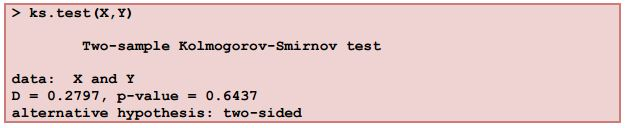
\includegraphics[width=0.99\linewidth]{KStest1}

\end{figure}

Remark: It doesn’t not suffice that both datasets are from the same distribution. They must have
the same value for the defining parameters. Consider the case of data sets; X and Z. Both are
normally distributed, but with different mean values.

\begin{figure}[h!]
\centering
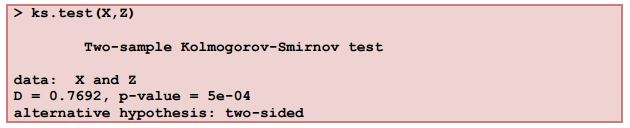
\includegraphics[width=0.99\linewidth]{KStest2}
\end{figure}



\subsection*{Kruskal-Wallis Test}
\begin{itemize}
\item The Kruskal-Wallis test is a nonparametric test used to compare three or more samples.
\item It is used to
test the null hypothesis that all populations have identical distribution functions against the
alternative hypothesis that at least two of the samples differ only with respect to location (median),
if at all.
\item It is the analogue to the One-Way Anova F-test used in analysis of variance. 
\item While analysis of variance tests depend
on the assumption that all populations under comparison are normally distributed, the Kruskal-Wallis
test places no such restriction on the comparison.
\item It is a logical extension of the Wilcoxon-Mann-Whitney Test.
\end{itemize}


\end{document}